\documentclass[12pt,A4paper]{article}
\usepackage[left=1.0in,top=1.0in,bottom=1.0in,right=1.0in]{geometry}
\usepackage{blindtext}
\usepackage{sectsty}
\usepackage{blindtext}
\usepackage{graphicx}
\usepackage{subfig}
\usepackage[english]{babel}
\sectionfont{\fontsize{12}{15}\selectfont}
\subsectionfont{\fontsize{10}{15}\selectfont}
\makeatletter
\renewcommand{\@seccntformat}[1]{%
	\ifcsname prefix@#1\endcsname
	\csname prefix@#1\endcsname
	\else
	\csname the#1\endcsname\quad
	\fi}
\addto\captionsenglish{
\renewcommand{\contentsname}
	{Table of Contents}
}
% define \prefix@section
\newcommand\prefix@section{}
\newcommand{\prefix@subsection}{}
\newcommand{\prefix@subsubsection}{}
\renewcommand{\thesubsection}{\arabic{subsection}}
\makeatother

\begin{document}
	\noindent
	Professor Spears, \\ \\
	\noindent
	Within the usability report of the Bridgestone tire changing guide you will find information breaking down the usefulness and purpose of the instructions provided by Bridgestone. Different methods were used when analyzing the document. A conclusion was found from the data collected.\\ 
	\\Our analysis included first looking over the document ourselves and giving our thoughts on the material provided. We used our insites to make decisions on how more information about the instructions would be collected. Interviews were conducted on eight different individuals, half having knowledge of changing tires and half that have never changed a tire before. These interviews provided insight on how useful, organized, and understanding the instructions were. It also allowed me to pin the intended audience. Knowing the intended audience gave information on who the document should be improved for. Two other instructions were found and each team member looked through and compared to the Bridgestone guide. Giving further insight on how the instructions could be improved.\\ 
	\\Any information regarding how data was tracked or findings from our information can be found in the document. The report goes over the entire process in detail, including our methods and resources.\\ \\Sincerely,\\ Group A
	\thispagestyle{empty}
	\clearpage
	\thispagestyle{empty}
	\begin{center}
		\Huge
		Usability Report of the Bridgestone Tire Change Guide \\
		\vspace{0.25 in}
		\Large
		 November 30, 2020 \\
		 \vspace{0.25 in}
		Written by: Carson Wille, Garrett Fields, Gavin Hamilton, Justin Pullman
		\begin{figure}[!h]
			\centering
			\vspace{0.5 in}
			\includegraphics[width=0.5\textwidth]{logo.jpg}
			\label{fig:f1}
			\caption{Bridgstone Logo}
		\end{figure}
		\vspace*{\fill}
		\section{Abstract}
	\end{center}
	\pagenumbering{roman}
	The Bridgestone tire change guide has incredible detail and is good at painting a picture of what needs to be done. However it is lacking in its abundance of pictures. This was confusing for some who had trouble picturing in their head what needed to be done. To assess this document we interviewed 8 subjects about their experience with the tire change guide. We asked them a series of questions assessing the qualitative properties of the document. We found many had around 60-70 percent retention rate when asked to describe how to change a tire after reading the document, and the subjects rated the website in aesthetics, how well the information was conveyed, and the overall organization of the document. On a scale of one to five the subjects gave the document an average rating of 4 for aesthetics, a 4.6 for conveyance of information, and a 4.75 for the organization of the document. We also compared the document with similar guides that come up when searching for a tire change guide, and the main differences were that the other websites had much more photos and one had videos that had step by step instructions.
	
	\clearpage
	
	\setcounter{page}{2}
	
	\tableofcontents

	
	\renewcommand\listfigurename{List of Illustrations}
	\listoffigures

	\clearpage
	\pagenumbering{arabic}
	\section{Executive Summary}

	\section{Introduction}
	
		\subsection{Subject}
		Changing a tire can be a tricky task and having a good set of instructions that are clear and easy to follow is important when on the side of the road trying to fix a car.

		\subsection{Purpose}

		\subsection{Background}
		The problem investigated by this paper is the usability of Bridgestone’s how to change a tire page on their website. The usability was tested in a variety of ways on different aspects of the website. The Bridgestone page was compared to other websites on how to change a tire by the writers of this paper. Along with the comparison to other websites, 8 test subjects were selected to answer questions about a wide variety of topics on the web page; this is covered in detail in the testing section. The usability of how to change a tire is very important as this is a situation that could happen to almost any driver.

		\subsection{Source}
		We gathered information by having eight subjects read the instructions and interviewing them over what they got out of the instructions and how useful it was to them. This allowed us to determine how the documents looks, understandability, and organization. We also made sure half the people interviewed have changed a tire before and half have not. This allowed us to compare and figure out who the target audience is. We also had each subject try to list every step they remembered to get an idea which group retained the most.

		\subsection{Scope}
		We researched the usefulness, simplicity, and organization of the document. We found a general target audience for the instructions and compared the understanding and usefulness to two other instructions of the same topic.

		\subsection{Significant Findings}
		Overall, the reception of the document was very strong. While individuals with prior experience understood the piece better, both individuals with and without tire changing experience rated their knowledge after reading the piece over 4 stars. This shows that the piece is effective overall and can be relied upon for clear and consistent direction.

		\subsection{Recommendations}
		We found a major thing that was lacking in the document was a lack of visuals. Pictures of each step or even videos would greatly improve the understanding and usefulness of this document. This would help the intended audience of people who haven't changed a tire to see all the parts and understand the process better.

		\subsection{Organization of Report}
		The document is split up into multiple sections. First, the document features a descriptive infographic of all the materials you will need, and categorizes them into items that should be included with your vehicle and items you will need to purchase separately. It then lists numbered steps to complete the tire change. This section unfortunately does not include any images for the reader to follow along with. The document concludes with a few other tips to handling the situation safely and effectively.

	\section{Methods}
	Eight subjects were selected to test the Bridgstone tire changing website. There was a set script of tasks and questions that each subject was asked to perform, this way there were consistent results with as little variables as possible. Four of our subjects were experienced at changing a tire, and four were not. To start the subjects navigated to the Bridgestone tire changing website by trying to search for it with their preferred search engine. They were then asked how that experience was and if there was any trouble navigating to the website. Then the subjects were told to read through the website in its entirety making note of anything that was confusing, or not immediately clear. After the subjects completed reading the document, they were asked to rate their experience in three areas: overall aesthetics of the website, how well the information was conveyed, and how well the document was organized. The rating system used was a one to five scale, one being the absolute worst they’ve seen and 5 being the absolute best. The document was then taken away from the subjects, and they were asked to write down as many steps in order they could remember. Lastly, they were asked if they learned anything from the document that they didn’t previously know. In addition to subject testing, we analyzed the website, comparing it with the other two links that appear when searching for “How to change a tire". 
	\vspace{1.6 in}
	\section{Results}
	\begin{figure}[!h]
		\centering
		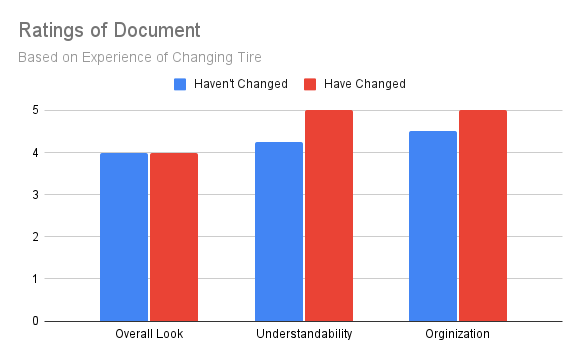
\includegraphics[width=0.65\textwidth]{Ratings_of_Document.png}
		\label{fig:f2}
		\caption{Ratings of the Document}
	\end{figure}
	Across the eight subjects we tested, four of them had changed a tire, and four of them had not. The first task, of navigating to the website, had some mixed results. Six of the subjects were able to find the website no problem, and two of the subjects needed a few tries and/or some guidance to get to the right website. For some search engines the Bridgstone website would not appear on the main page and the subject would need to scroll down. After the subjects read through the document, they were asked to rate various aspects of the website. A 1 is a very poor score, and a 5 is an excellent score. On overall aesthetics we had an average score of 4. For overall comprehension/clarity of the website there was an average score of 4.6. The clarity depended on whether the subject had experience changing a tire. Among the subjects who had changed a tire previously, there was a clarity rating of 5. And among those who had not changed a tire the clarity rating was a 4.25. The overall organization of the document was rated at 4.75. This rating was also split amongst those who had experience and those who had no experience. The ratings respectively were 5 and 4.5. When asked if there were any clarity issues our subjects responded that for the most part they understood what the author was trying to convey. One of our subjects had some trouble with the jargon, some of the parts were foreign names to them. And one of our subjects was confused by the required and optional parts. The optional parts were used in the instructions and were taken to mean that they weren’t really optional. We took the document away and asked the subjects to write down as many steps as they could remember in order, and found that on average they remembered 70\% of the steps. The standard deviation of the retention levels is 11.6\% with our range being from 61\% to 89\% retention. As we compared the documents to both the Home Depot and WikiHow site, many of us had drawn the same conclusion. The Bridgestone site has great information but lacks any visuals which can be confusing for readers inexperienced with cars. Both Home Depot and Wikihow included pictures with each step to show roughly what was happening whereas Bridgestone just had a large wall of text which can be hard for readers to understand, or in some cases even bore the reader.

	\section{Conclusions}

	\section{Recommendations}
	The main issue with Bridgestone’s How to Change a Tire webpage is the lack of visuals. The information presented is very thorough, but the lack of a visual for people unfamiliar with cars can leave readers confused. The data is also presented as a wall of text, visuals could be used to help break this up to make the website more appealing to a reader rather than just looking at a giant block of information. More specifically Bridgestone should include a picture of what is being done for each step so readers can use the detailed text to the best of their ability and then reference the visuals when there is any confusion. As mentioned in the results one subject did not understand what a lug nut was, a visual of what was being done on the tire could have easily resolved the reader's confusion. This one simple change would greatly increase the usability of this website. 

	\section{References}
	“How to Change a Flat Tire.” Bridgestone Tires, 29 Nov. 2021, https://www.bridgestonetire.com/learn/maintenance/how-to-change-a-flat-tire/.\\ \\
	“How to Change a Tire.” The Home Depot, https://www.homedepot.com/c/ah/how-to-change-a-tire/9ba683603be9fa5395fab908e21cabb.\\ \\
	“How to Change a Tire.” WikiHow, WikiHow, https://www.wikihow.com/Change-a-Tire.\\

\end{document}